\section{Fundamentals of architecture}

\subsection{Introduction}

Inside a computer, a processor executes instructions.
\begin{itemize}
    \item \textbf{Fetch/Decode}: Determine which instruction to run next;
    \item \textbf{ALU} (execution unit): Performs the operation described by an instruction, which may change values in the processor's registers or the computer's memory;
    \item \textbf{Registers}: maintain program state, store values of variables used as inputs and outputs to operations.
\end{itemize}
The simplest and most basic processor executes \textbf{one instruction per clock cycle}.
\begin{figure}[!htp]
    \centering
    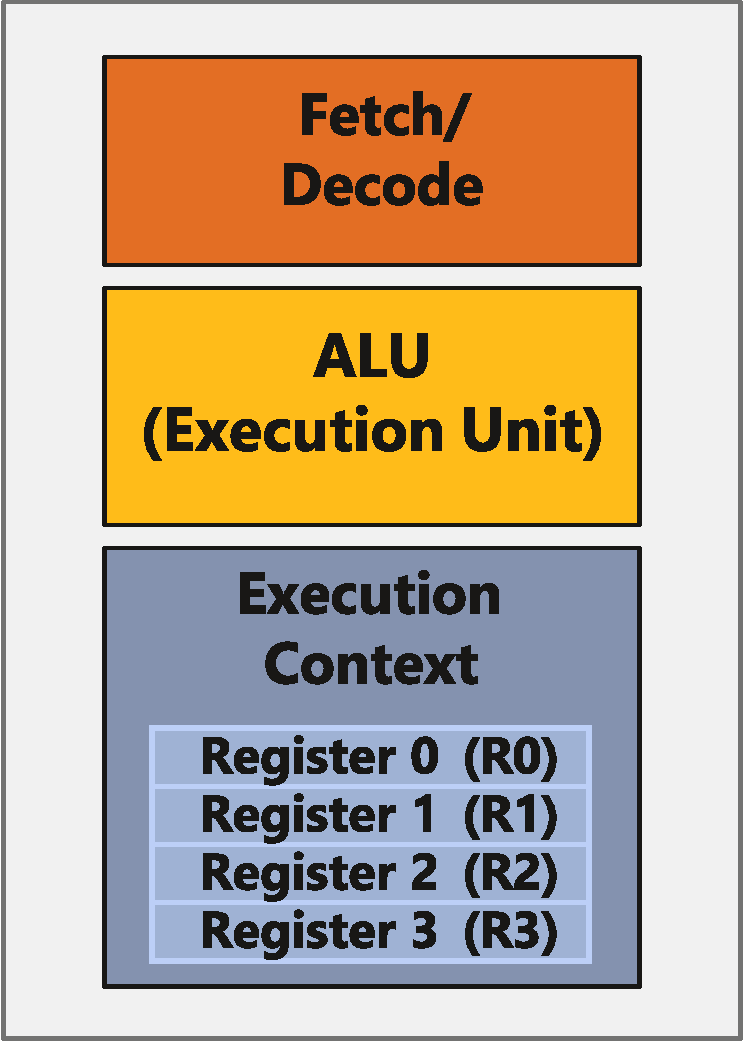
\includegraphics[width=.24\textwidth]{img/simplest-prcoessor-1.pdf}
    \caption{The simplest and most basic processor.}
\end{figure}

\noindent
A more \dquotes{complex} and realistic model is the \definitionWithSpecificIndex{superscalar processor}{Superscalar Processor}. This \textbf{processor can decode and execute up to \underline{two instructions per clock}}. The execution is slightly different from the simplest processor. The \textbf{processor automatically finds independent instructions in an instruction sequence and can execute them in parallel on multiple execution units}.
\begin{figure}[!htp]
    \centering
    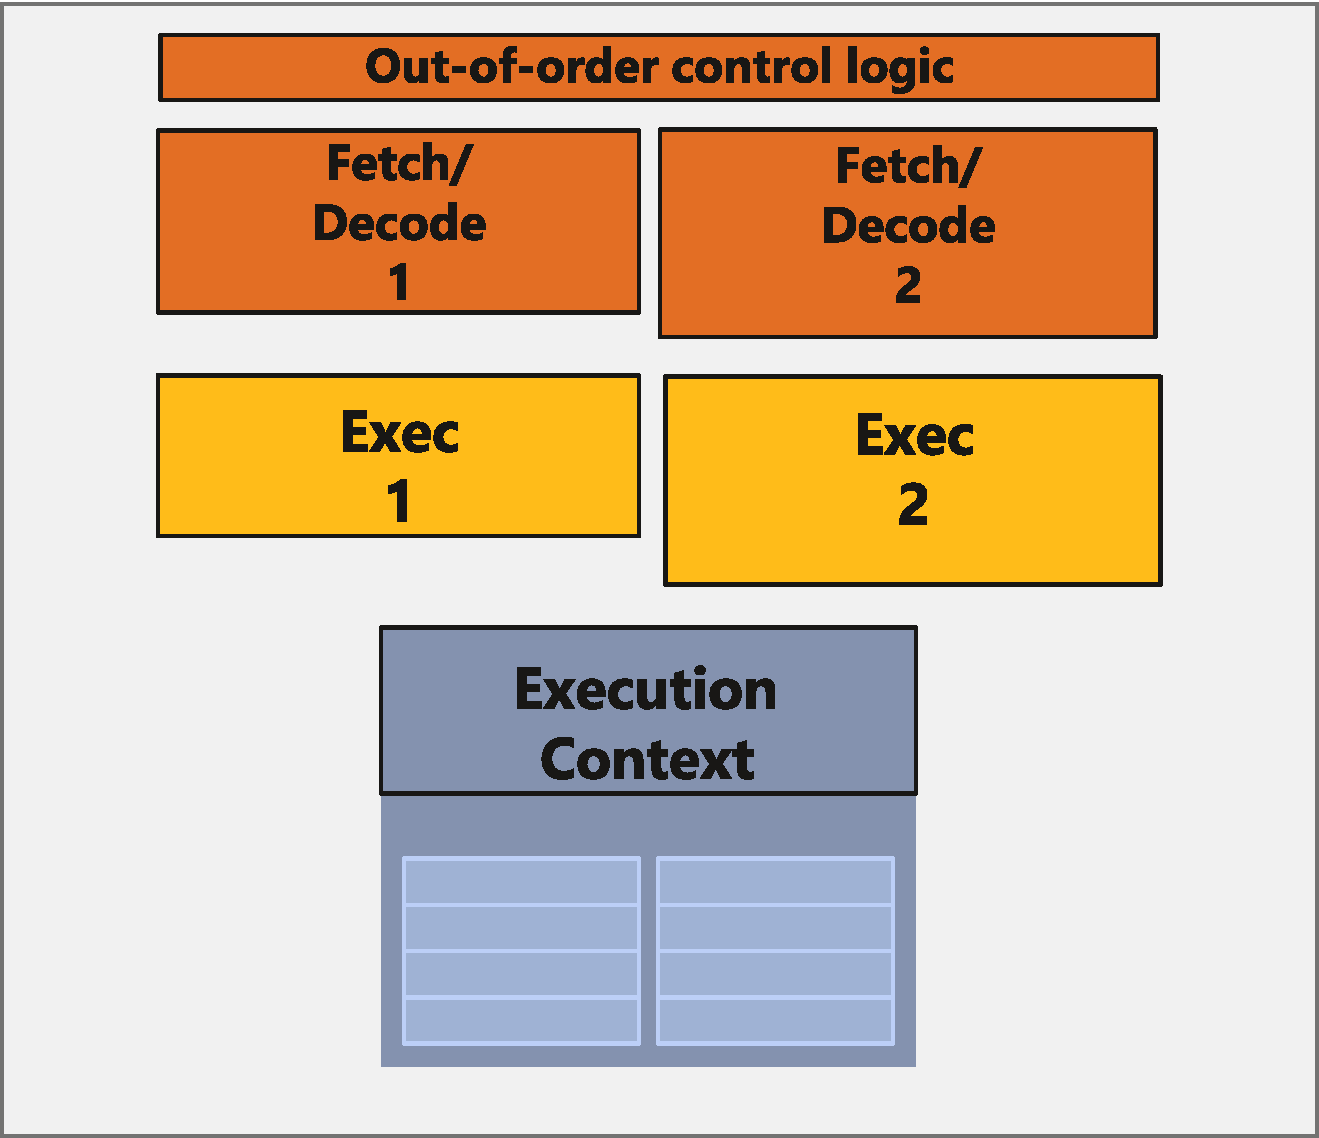
\includegraphics[width=.52\textwidth]{img/superscalar-prcoessor-1.pdf}
    \caption{The superscalar processor.}
\end{figure}